\chapter{Two level graph matching} \label{chapter:2levelGM}
In this chapter we describe our novel approach for graph matching. Our aim however was not to develop a new matching algorithm, but to propose a framework, which would help to solve problems, where the direct application of existing matching algorithms is impossible due to memory requirements or runtime. This is often the case when a graph matching problem is formulated using a similarity matrix between graphs~(see Eq.~\eqref{eq:gQAP1}). The main idea of our approach is based on the \emph{divide and conquer} technique~\cite{Cormen}, which is well known from its application for array sorting algorithms. According to this general paradigm, a given graph matching problem, which is too difficult to be solved directly, is subdivided into smaller subproblems. Those subproblems are created in such a way, that they can be solved without great effort. A resulting solution is then combined from local solutions of single subproblems. A disadvantage of such an approach is however, that a runtime improvement is sometimes paid with a drop in the accuracy.
Due to that, one want to have a trade off between speed up and accuracy. What is more important depends on a particular problem.

Several existing algorithms share similar ideas. Those which are closest to our approach were described in the previous chapter under the group of algorithms based on clustering techniques. Below we review them shortly again to point out, that none of them is completely repeated by our framework.

This chapter is organized as follows. First of all we formulate a considered graph matching problem and show some issues of this formulation. In the second part, we describe our two level graph matching framework, which should help to cope with the formulated problems. The performance results and comparison with other algorithms are summarized in the next chapter. 
% ---------------------------------       Problem Statement      -------------------------------------
\section{Problem statement} \label{sec:prob_stat}
Consider two attributed graphs $G^I = (V^I, E^I, D^I)$ and $G^J = (V^J, E^J, D^J)$, where $V^{I(J)}$, $E^{I(J)}$, $D^{I(J)}$ denote set of nodes, set of edges and set of node attributes respectively. We assume the situation, where those graphs are undirected and do not have multiple edges between nodes. Let the size of the first graph be $n_1$ and the second $n_2$. Without loss of generality, we assume that $n_1\le n_2$. Attributes of the graphs are $r-$dimensional real vectors: $D^I,D^J\in\mathbb{R}^r$.

We define a problem of matching two graphs $G^I$, $G^J$ as a quadratic assignment problem (same formulation as Eqs.~\eqref{eq:gQAP1}-\eqref{eq:gQAP4}). 
\begin{alignat}{2}
    &     && \argmax_x{x^TSx}                           \label{eq:gQAP1_2}\\
    & \text{s.t. } &&  x\in \{0,1\}^{n_1n_2}            \label{eq:gQAP2_2}\\
    &             &&  \sum_{i=1\dots n_1} x_{ij}\le 1   \label{eq:gQAP3_2}\\
    &             &&  \sum_{j=1\dots n_2} x_{ij}\le 1   \label{eq:gQAP4_2}
\end{alignat}
We denote a pair of nodes $(v_i,v_j)$, where $v_i\in V^I$ and $v_j\in V^J$, as a correspondence between the sets $V^I$ and $V^J$. Let $M$ be a set of all possible correspondences between the nodes of the graphs $G^I,G^J$. Obviously, $M$ consists of $n_1n_2$ node pairs.  Then the vector $x\in \{0,1\}^{n_1n_2}$ is an indicator vector of a subset $m=\{(v_i,v_j)|v_i\in V^I,v_j\in V^J\}$ of the set $M$. This means, that element $x_k$ of this vector is equal $1$ if and only if the corresponding k-th node pair $(v_i,v_j)$ is selected into subset $m$. The constraints~\eqref{eq:gQAP3_2},~\eqref{eq:gQAP4_2} ensure, that each node of the graph $G^I$ is matched to exactly one node of the second graph $G^J$.

The matrix $S\in\mathbb{R}^{n_1n_2\times n_1n_2}$ in Eq.~\eqref{eq:gQAP1_2} encloses the precomputed information about similarity of two graphs. Rows (columns) of this matrix correspond to the elements in the set $M$ of all possible node correspondences. Its diagonal elements $S_{kk},k=1,\dots,n_1n_2,$ contain similarity measurements of the node pairs $(v_i,v_j)\in M$. The non-diagonal elements measure similarity of edges between two pairs of matched nodes. Our aim is to find maximal $n_1$ correspondences between the nodes of the graphs $G^I,G^J$, which maximizes the similarity value between those graphs.

As we saw in the previous chapter, the selected formulation of a graph matching problem is widely used as the most general one. However, the size of the affinity matrix $S$ can cause problems due to the required memory demands. For example, a dense affinity matrix between two graphs with $200$ nodes each needs approximately 12Gb memory (double precision). There are several possible ways to reduce the memory complexity of the formulated graph matching problem. Here we mention three possible approaches.

The first one is to reduce a set of candidate correspondences by selecting a subset $M^\prime\subset M$. This can be done, for example, by restricting the number of candidate matches for a node $v_i\in V^I$ to some number smaller than $n_2$. This method is often used, as it not only solves memory issues of the problem formulation as defined in Eqs.~\eqref{eq:gQAP1_2}-\eqref{eq:gQAP4_2}, but also reduces the algorithmic complexity of many algorithms, which highly depend on the number of possible matches~(e.g.~\cite{Cho2014_Haystack,Cho2010_RRWM,Cho2012_ProgressiveGM, Leordeanu2005_SM}).

The second possibility, is to make the matrix $S$ sparser by excluding the comparison of some nodes or edges from the consideration. In case of big graphs this can however lead to a high loss of initially provided information and influences dramatically the quality of a resulting matching. 

The third possibility is to replace the initial problem of graph matching by a set of smaller subproblems, that arise by partitioning given graphs into subgraphs and matching those subgraphs. It means, that the matrix $S$ is divided into blocks, where each block represent a similarity matrix between two subgraphs. Thereby the similarities of edges, whose nodes belong to different subgraphs after problem splitting, will be ignored. \ToDo{On the one hand, this approach solves the memory problem by replacing the initial matrix $S$ with a set of smaller affinity matrices}. On the other hand, it does not necessary reduce the time complexity of the initial problem, as selection of correspondences between subgraphs means in the worst case their pairwise matching in all possible combinations. Otherwise, further information will be lost. Despite the mentioned drawbacks, the single subgraph matching problems can be eventually parallelized, that still makes the approach attractive to be applied on big graphs.

In the framework for graph matching, that we describe in detail below, we use the third of the described techniques. We divide given initial graphs into subgraphs and iteratively search first for correspondences between the subgraphs and then for node correspondences between matched subgraphs. For subgraph matching we use an existing matching algorithm. A graph partitioning is performed only at the initialization step, but after each iteration subgraphs have a chance to exchange nodes on their borders.

To our best knowledge the described method was not published before. Especially, we haven not seen an iterative graph matching algorithm based on graph clustering so far, which updates initial partitions. At the same time there is a certain overlap in ideas between our and existing works. The algorithm proposed by Lyzinski et al.~\cite{Lyzinski2015} uses graph partitioning to parallelize a semi-supervised graph matching problem, where some correspondences between graph nodes are provided. The graph matching problem is formulated as the minimization problem~\eqref{eq:QAP1}, that does not use an affinity matrix $S$. The given matches between graph nodes are used to cluster two graphs jointly and to find correspondences between subgraphs. As a consequence, subgraphs of given graphs are similar enough to ensure the matching quality. However the proposed clustering method cannot be used for an unsupervised matching.

An idea similar to our one to use graph partition for graph matching in unsupervised cases was used by Carcassoni and Hancock~\cite{Hancock_ModalClusters}, Qui and Handcock~\cite{Hancock_GM_SpectralPart} and recently by Nie et al.~\cite{CliqueGraph_CVPR2015}. From them only the algorithm by Nie et al.~\cite{CliqueGraph_CVPR2015} considers the same maximization problem as we do. The two other algorithms formulate the graph matching problem in terms of relaxation labeling. Also the definition of the graph clusters differs between the algorithms. Qui and Hancock, as well as Nie et al., consider clusters, that are built by direct neighborhoods of nodes. The resulting partition can be overlapping~\cite{CliqueGraph_CVPR2015} or not~\cite{Hancock_GM_SpectralPart}. Our algorithm and the one in the paper of Carcassoni and Hancock~\cite{Hancock_ModalClusters} consider the more general case, where a graph partition is given by a disjoint set of arbitrary subgraphs of a graph.
Finally, similar to our approach Qui and Handcock~\cite{Hancock_GM_SpectralPart} use the extracted graph partitioning to create a new graph, whose nodes represent clusters of the initial graph. They call this process graph simplification. However their approach quite differs from ours, because of the special definition of clusters, another problem formulation and a different approach for solving the single matching problems, as we mentioned in the previous chapter.

In the remainder of this chapter we describe in detail our graph matching framework.

% ---------------------------------------    Approach       ------------------------------------------
\section{Two level graph matching algorithm}
For simplicity we consider at the beginning only one graph $G^I=(V^I,E^I,D^I)$ of size $n_1$. Assume, that we know a partition of the node set $V^I$ of this graph into $m_1$ non-overlapping clusters based on some rule: $V^I=\cup_{k=1}^{m_1}V^I_k$, where $V^I_{k_1}\cap V^I_{k_2}=\emptyset$ for $k_1\not=k_2$. Based on this partition the initial graph $G^I$ is subdivided into a set of node induced subgraphs $\{G[V^I_k]\}_{k=1}^{m_1}$. Note, that it holds $G[V^1]\cup\dots\cup G[V^{m_1}]\subset G^I$, because edges between different subgraphs are not presented in the left union.
Further, we define a mapping $U$ between the set of graph nodes $V^I$ and another set of nodes $V^{Ia}=\{a_k\}_{k=1}^{m_1}$, where a single node $a_k$ represents a subgraph  $G[V^I_k]$. This mapping can be expressed as an matrix $U^{Ia}\in\{0,1\}^{n_1\times m_1}$ with elements 
\begin{equation}\label{eq:matrixU}
U^{Ia}_{ik} = \begin{cases} 1, & \mbox{if node } v_i\in V^I_k,    \\
0, & \mbox{otherwise}.\end{cases}
\end{equation}
The new set $V^{Ia}$ defines a node set of a new graph built on top of the other one. A pair of new nodes $a_{k_1},a_{k_2}\in V^{Ia}$ is connected with an edge if and only if there is at least one edge in the initial graph $G^I$ between the corresponding clusters $V^I_{k_1}$ and $V^I_{k_2}$. The set $V^{Ia}$ together with the set of edges between its elements and correspondence matrix $U^{Ia}$ builds a new graph $A^I=(V^{Ia},E^{Ia},U^{Ia})$. We will call the graph $A^I$ an \emph{anchor graph} of the graph $G^I$ and its nodes \emph{anchor nodes} or just \emph{anchors}. The graph $G^I$ together with its anchor graph $A^I$ builds a two level system: the graph $G^I$ is located on the lower (finer) level and the graph $A^I$ on the higher (coarser) level (see Fig. \ref{fig:2levels}).

\begin{figure} [h!]
	\centering
	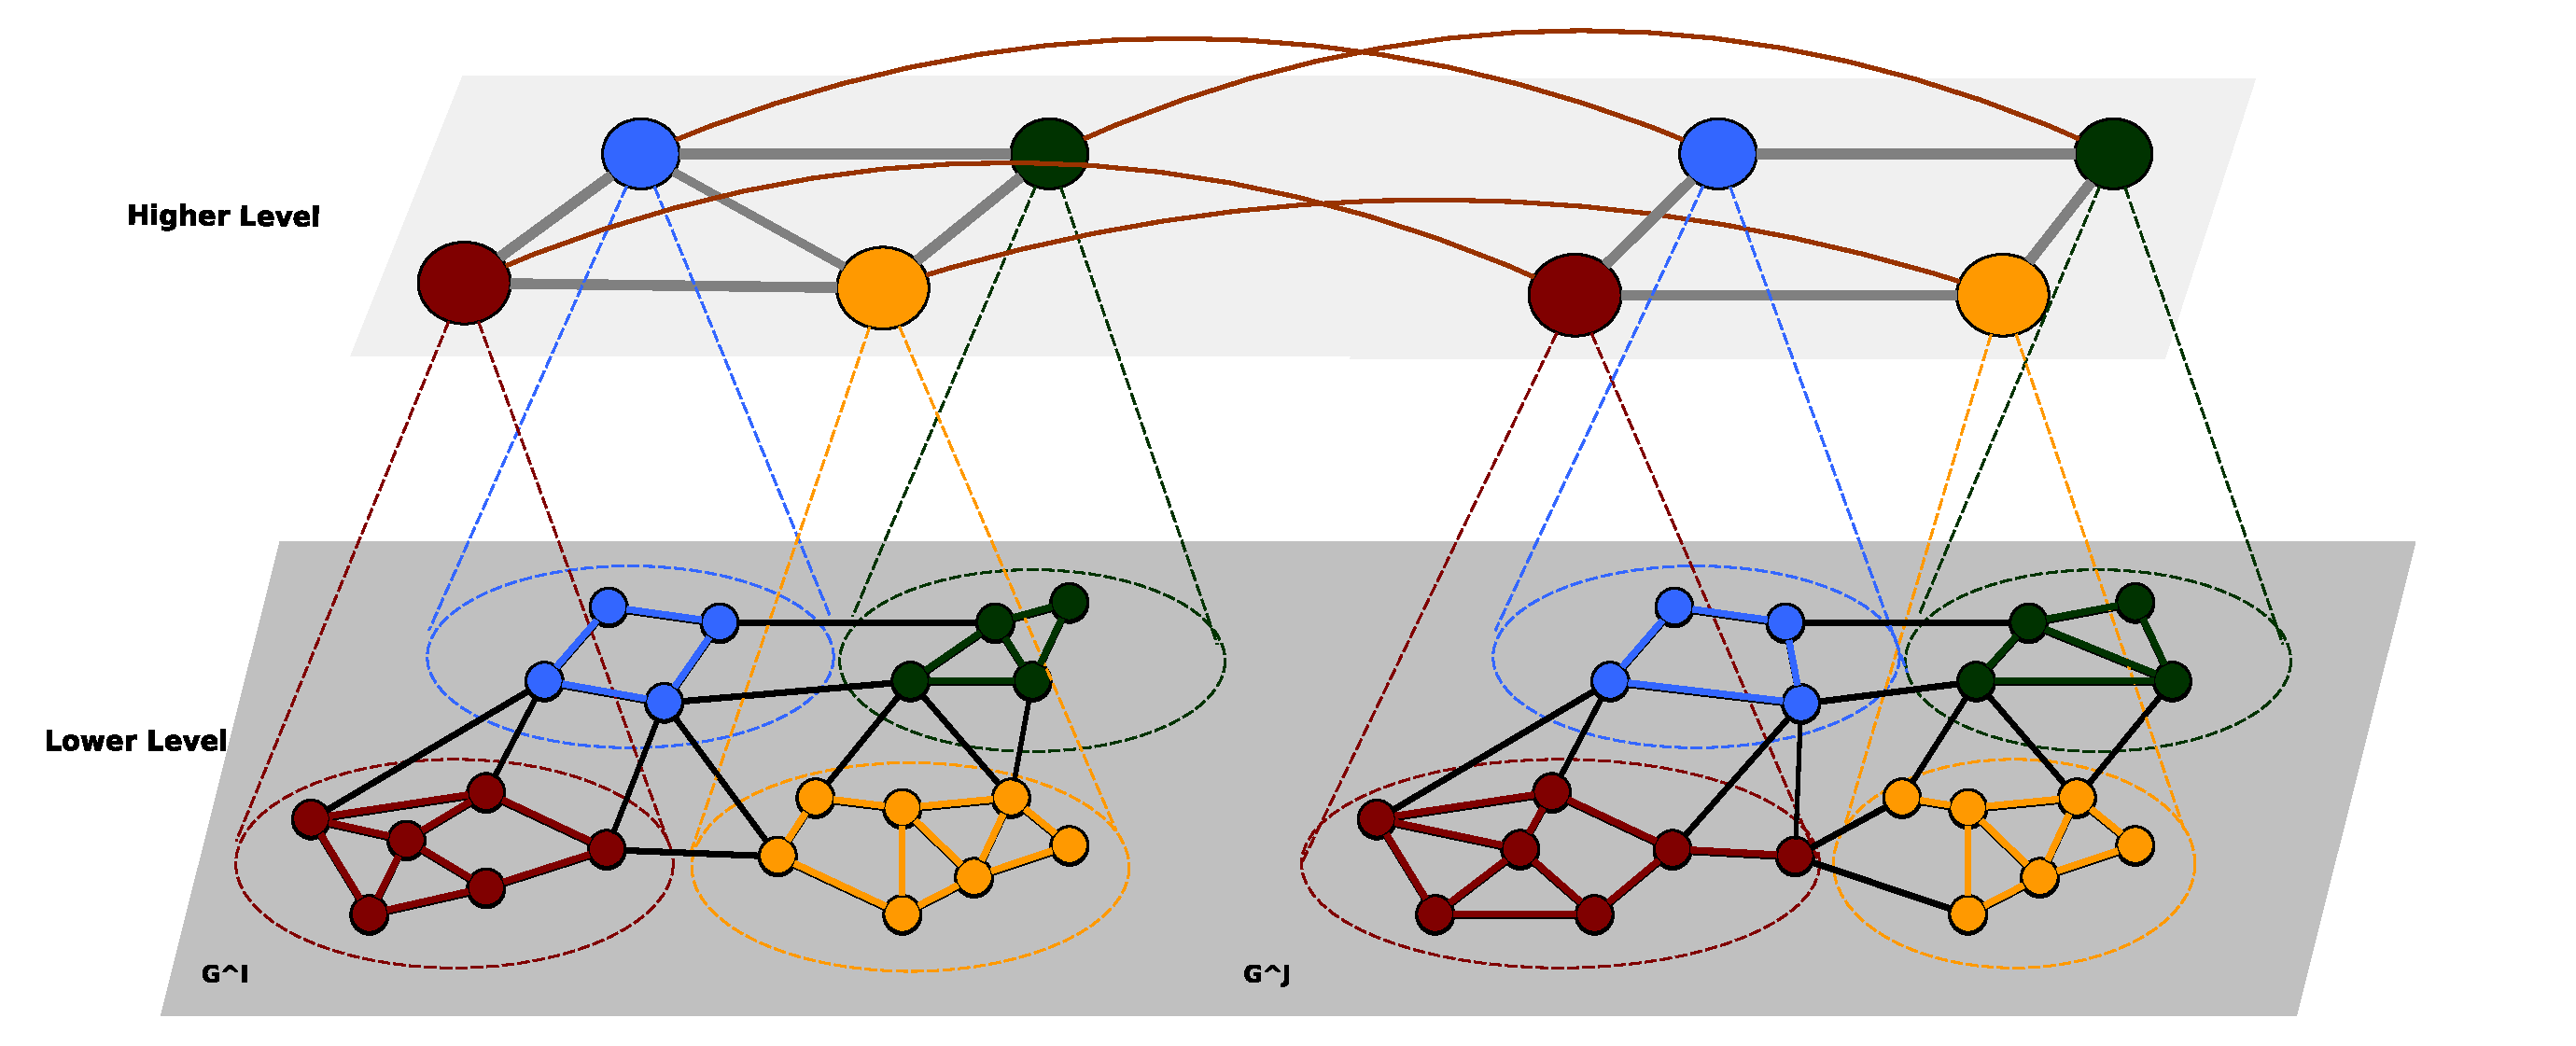
\includegraphics[scale=0.35]{chapter2/fig/twolevels3.pdf}
	\caption{Two level framework for graph matching} \label{fig:2levels}
\end{figure}

We return now back to the case of two graphs $G^I=(V^I,E^I,D^I)$ and $G^J=(V^J,E^J,D^J)$, which we want to match. 
For each of them we build an anchor graph $A^I=(V^{Ia},E^{Ia},U^{Ia})$ and $A^J=(V^{Ja},E^{Ja},U^{Ja})$ respectively.
Now instead of matching graphs $G^I$ and $G^J$ directly on the lower level, we want to match first the corresponding anchor graphs. Matches between anchor nodes give us correspondences between underlying subgraphs. After that, we can perform graph matching for each pair of matched subgraphs independently. A union of local solutions from the single subgraph matching problems gives us a solution of the initial problem. More formally, we replace the objective function of the initial matching problem (see Eq.~\eqref{eq:gQAP1_2}, \eqref{eq:sumQAP}) with the new function:
\begin{equation}\label{eq:sumQAP_2}
	S(G^I,G^J,m|m^a)=\sum_{\substack{ v_{i},v_{i^\prime}\in V^I_k\\v_{j},v_{j^\prime}\in V^J_p\\ m^a(a_k)=a_p}}s_E(e_{ii^\prime},e_{jj^\prime}) + \sum_{\substack{ v_{i}\in V^I_k\\v_{j}\in V^J_p\\ m^a(a_k)=a_p}}s_V(v_{i},v_{j}),
\end{equation}
where $S(G^I,G^J,m|m^a)$ denotes the similarity of the initial graphs given the matching $m^a=\{(a_k,a_p)|a_k\in A^I,a_p\in A^J\}$ of the corresponding anchor graphs or, which is the same, the correspondences $\{(V^ I_k,V^J_p)|V^I_k\subset G^I,V^J_p\subset G^J\}$ between the subgraphs of the initial graphs.

Why can this approach be better than the direct one? As we cab see from the previous section the time and space complexity of the considering graph matching problem depends highly on the size of initial graphs. Constructed anchor graphs are however several time smaller than the initial graphs, which means, the matching algorithm on the anchor level can be performed much faster and without high memory demand compared to the lower level. The same holds true for matching between the subgraphs.
%If $C(n)$ is complexity of a graph matching algorithm with $n$ possible correspondences.
Obviously, the accuracy of such an two level matching approach depends heavily on the partition of the initial graphs into subgraphs and on the quality of a graph matching algorithm on both the higher and lower levels. We concentrate ourself on the first of this two critical moments and use an existing algorithm for graph matching. To make the described two level approach more robust against graph partitioning we suggest to use an obtained matching between two graphs to correct their partitions. The overall procedure (matching on the higher level, matching on the lower level and partition updating) is then repeated iteratively till convergence of the objective function~\eqref{eq:gQAP1_2}. The algorithm is summarized below in Alg.\ref{alg:2levelGM}.

\begin{algorithm}[h]
	\KwIn{ initial graphs $G^I$, $G^J$\\
		   \hspace{45pt}maximal number of iterations $N$\\
		   \hspace{45pt}convergence parameters $R$ and $\epsilon$}
	\KwOut{set $m$ of correspondences between the nodes $V(G^I)$ and $V(G^J)$}
	construct anchor graph $A^I$ of the graph $G^I$ \label{alg:2levelGM_clustering1}\\
	construct anchor graph $A^J$ of the graph $G^J$ \label{alg:2levelGM_clustering2}\\
	i=0, $score_i$=0\\
	\While{$r<R$  \textbf{AND} $i\le N$}
	{ $i=i+1$ \\
	  \If{$i\ge 2$}
	  {update subgraphs $G[V^I_k],G[V^J_p],k=1\dots,m_1,\ p=1\dots,m_2$ \label{alg:2levelGM_update}}
	  match anchor graphs $A^I$,$A^J$ \label{alg:2levelGM_GM1} \\
	  $m_i=\emptyset$\\
	  \ForEach{pair of matched anchors $(a_k,a_p),a_k\in V(A^I), a_p\in V(A^J)$}
	  {match subgraphs $G[V^I_k]$,$G[V^J_p]$ \label{alg:2levelGM_GM2}\\
	   $m_i=m_i\cup\{m^k_i\}$\hspace{55pt}\tcc{$m^k_i$ set of local correspondences}
	  }
	  $score_i=x^TSx$\ \ \tcc{$x$ the indicator vector of the subset $m_i\subseteq M$}
	  \If{$|score_i-score_{i-1}|<\epsilon$}
	  {$r=r+1$}
	  \Else{$r=0$}
	}
	\Return $m_i$
	\caption{twoLevelGM($G^I$, $G^J$, $N$, $R$, $\epsilon$)} \label{alg:2levelGM}
\end{algorithm}

In the following we describe in detail the single steps of our approach: %initial graph construction,
graph partitioning~(lines~\ref{alg:2levelGM_clustering1},\ref{alg:2levelGM_clustering2}), graph matching algorithm on both levels~(lines~\ref{alg:2levelGM_GM1},\ref{alg:2levelGM_GM2}), as well as the update rule for current graph partitions~(line~\ref{alg:2levelGM_update}).
%\FloatBarrier
% ---------------------------------------        HLG Construction
\subsection{Anchor Graph Construction}
The problem of anchor graph construction for initially given graph $G^I=(V^I,E^I,D^I)$ turns straight forward into a problem of partitioning the graph $G^I$. During our work on this thesis we tried out different strategies for clustering nodes of a given graph. Here we present those, which were more suitable for our matching framework, however generally an arbitrary algorithm for graph partitioning can be used.

Here and further we assume that the nodes of the given fine graph $G^I$ are located on a plane. That means, for each node we have additionally to its attribute an associated pair of coordinates and therefore can define the length of an edge as a $L^2-$distance between its endpoints. The reason for this assumption is given by practical applications such as image or object recognition.
\subsubsection{Using grid}	
The first algorithm we describe is the most simple one. It uses a grid with fixed number of rows $r$, columns $c$ and a cell width $w$. The grid is placed over the graph $G^I$. Nodes, that are captured by a same grid cell belong to one cluster. Obviously, the number of clusters is equal to $r\times c$. We place anchor nodes in the middle of the grid cells. Two anchors are connected by an edge, if the cells they belong to have a common edge.
\subsubsection{Algorithms based on node merge}
The next considered approach creates an anchor graph $A^I$ with a predefined number $m_1$ of anchors. For that we adopted a coarsening phase from multi-level graph partition algorithms \cite{Chevalier09_GP, Safro2012_GC, Karypis95_GP, Hendrickson1995}.
Such algorithms have generally three phases: 
\begin{enumerate}
	\item graph coarsening phase, where one creates a hierarchy of graphs by successive merging of nodes in graph on previous stage starting with initial graph;
	\item graph partition phase, where the partition problem is solved exact on the coarsest level;
	\item refinement phase, where solution of the coarsest level is interpolated through all levels of the hierarchy until the initial graph.
\end{enumerate}
There are several types of graph coarsening algorithms. In our work we used so-called strict aggregation scheme (SAG)~\cite{Chevalier09_GP}, which groups nodes of $G^I$ in disjoint subsets based on the strength of the edges between them. We implemented two SAG based algorithms: Heavy Edge Matching (HEM) and Light Edge Matching (LEM)~\cite{Chevalier09_GP}. Both algorithms visit nodes of the graph $G^I$ in random order and construct an independent set of edges $E^\prime$ of the graph. The edge selection is based on the edge weights. The HEM picks and adds into $E^\prime$ the strongest edge adjacent to a current node $v$, that does not belong to the set of end nodes of edges in $E^\prime$~(see Alg.~\ref{alg:HEM}). As opposed to this, the LEM selects the weakest edge adjacent to a current node. The edges in $E^\prime$ will be contracted, i.e. their endpoints will be replaced with a new node, that lies in the middle of a contracted edge and is connected to all neighbors of its endpoints.

%{\LinesNumberedHidden
%\LinesNumberedHidden
%\LinesNotNumbered
\begin{algorithm}[h]
	i = 0, $E^\prime=\emptyset$ \\
	\While{$|V(G^I)|>m_1$  \textbf{AND} $i\le N$}
	{ select a random node $v\in V(G^I)\setminus V(M)$ \\
	  \If{$\exists v^\prime=\argmax_{u\in V(G^I)\setminus V(M)} w(v,u)$}
	  {$E^\prime=E^\prime\cup{e_{vv^\prime}}$}
	  \Else{$i=i+1$}
	}
	\Return $G^I$
	\caption{HEM($G^I$, $m_1$, $N$)} \label{alg:HEM}
\end{algorithm}

In our case, the graph $G^I$ is not initially weighted. To use the described coarsening methods we need to define a strength of graph edges. In case of LEM-Algotihm we set the length of an edge as its strength: $w_{vv^\prime}=\|v-v^\prime\|_{2}$. If we use HEM-Algorithm the strength of an edge is equal to $w_{ii^\prime} = exp(-\frac{\|v-v^\prime\|_{2}}{\sigma^2_{s}})$ with a constant $\sigma^2_{s}$.

It is clear, that one iteration of HEM or LEM reduces the number of nodes in $G$ at most by $\lfloor\frac{n}{2} \rfloor$ nodes. To get an coarse graph with $m_1$ nodes the coarsening algorithm should be repeated several times.

\subsection{Anchor graph matching}
In the previous section we described how to construct anchor graphs $A^I=(V^{Ia},E^{Ia},\newline U^{Ia})$ and $A^J=(V^{Ja},E^{Ja},U^{Ja})$ of given graphs $G^I = (V^I, E^I, D^I)$ and $G^J=(V^J, E^J, D^J)$ respectively. Now, we focus our attention on the problem of matching two anchor graphs. For that, according to our problem formulation (see Eqs.~\eqref{eq:gQAP1_2}-\eqref{eq:gQAP4_2}), we need to define a similarity matrix $S^A\in\mathbb{R}^{m_1m_2\times m_1m_2}$ between the graphs $A^I$ and $A^J$, where $m_1=|V^{Ia}|$ and $m_2=|V^{Ja}|$. This matrix contains two types of similarities: edge similarities (non-diagonal elements) and node similarities (diagonal elements).

Let us consider a pair of anchors  $a_k$, $a_k^\prime\in V^{Ia}$. We define the length of the edge $e_{kk^{\prime}}$ between those anchors as a median of distances between nodes in the corresponding subgraphs $G[V^I_k]$ and $G[V^I_{k^\prime}]$. With other words:
\begin{equation} L_{kk^\prime} = \median_{\substack{v_i\in G[V^I_k]\\ v_{i^\prime}\in G[V^I_{k^\prime}]} }\|v_i-v_{i^\prime}\|_{2}. \end{equation}
%where $\|v_i-v_{i^\prime}\|_{2}$ is the euclidean distance between the nodes $v_i\in G[V^I_k]$ and $v_{i^\prime}\in G[V^I_{k^\prime}]$.
Using this definition we calculate the similarity $s^A_E(e_{kk^\prime}, e_{pp^\prime})$ between the edges $e_{kk^\prime}\in E^{Ia}$ and $e_{pp^\prime}\in E^{Ja}$ based on their length as it was done in Eq.~\eqref{eq:edge_sim1}:
\begin{equation*}
s^A_E(e_{kk^\prime}, e_{pp^\prime}) = exp(-\frac{(L_{kk^\prime} - L_{pp^\prime})^2}{\sigma^2_{s}}).
\label{eq:s_e_A}
\end{equation*}

As we already discussed in the previous chapter, a natural way to define node similarities is to compare their attributes. However, our anchor graphs $A^{Ia}$ and $A^{Ja}$ do not have direct attributes in contrast to the initial graphs $G^I$, $G^J$. Further we describe two ideas, how to work around this problem. %which we suggest to calculate anchor similarities.

The first idea is to assign some attributes to the anchors and proceed further in the same way, as for the initial graphs. However, if we define those attributes based only on the anchor graphs without involving the provided information about underlying initial graphs, the overall matching result can be corrupted. The reason for this is, that an anchor in one graph can get a similar attribute, as an anchor from the other graph, although those anchors represent different subgraphs in the original graphs. If they will be selected by the matching algorithm, the matching of the underlying subgraphs will have very low quality. This will have in turn an impact on the quality of the total matching of initial graphs. Consequently anchor attributes should incorporate the information about underlying subgraphs of original graphs.
Consider an anchor $a_k\in V^{Ia}$ and its underlying subgraph $G[V^I_k]=(V^I_k,E^I_k,D^I_k)$. We suggest two classes of attributes of the anchor $a_k$. 
\begin{itemize}
\item The first one uses node attributes $D^I_k$ of the underlying subgraph $G[V^I_k]$. For this purpose we adopted the \emph{bag of features model}~\cite{BoF_Leung2001}. We build once a common dictionary of all provided attributes in the two fine graphs by performing \emph{k-means clustering} of $D^I\cup D^J$ into $C$ clusters. The centers of the clusters represent "codewords". Each attribute of a node in $V^I_k$ is afterwards mapped onto the closest codeword. In this way, the anchor attribute $d_1(a_k)\in\mathbb{R}^C$ is defined as normalized histogram of "codewords" in the corresponding subgraphs.

\item The second class of attributes should capture the geometrical structure of underlying subgraph. We define $d_2(a_k)\in\mathbb{R}^{|V^I_k|\times b}$ as a set of $|V^I_k|$ histograms $\{d_2(a_k,v)\}$ with $b$ bins. Each histogram $d_2(a_k,v)$ represents a distribution of the length of the subgraph edges inside a small circle region around a node $v\in V^I_k$. 
\end{itemize}
The similarity value between two anchors can now be determined based on the first or second type of anchor attributes. To calculate a distance between histograms we use $\chi^2$ statistic test \cite{Weken2004_ChiSqTest}:
\begin{equation}
s^A_1(a_k, a_p) = \sum_{b_i\in B}\frac{(d_1(a_k,b_i)-d_1(a_p,b_i))^2}{(d_1(a_k,b_i)+d_1(a_p,b_i)},
\end{equation}
\begin{equation}
s^A_2(a_k, a_p) = \frac{1}{|V^I_k|}\frac{1}{|V^J_p|}\sum_{v\in V^I_k}\sum_{u\in V^J_p} \big(\sum_{b_i\in B}\frac{(d_2(a_k,v,b_i)-d_2(a_p,u,b_i))^2}{(d_2(a_k,v,b_i)+d_2(a_p,u,b_i))}\big),
\end{equation}
where $a_k\in A^I, a_p\in A^J$ and notation $d_1(a_k,b_i)$ and $d_2(a_k,v,b_i)$ denote a value in the $b_i$-th bin of the corresponding histogram. 
Both defined similarities can be used separately or set together as a linear combination into one similarity function.

The second idea to determine similarity $s^A(a_k, a_p)$ between two anchors is to perform graph matching of the underlying subgraphs $G[V^I_k]$, $G[V^J_p]$ and take its score as a similarity measure. This idea has a great drawback of high computational complexity, because we need to perform in total $m_1m_2$ local matches. However, in this case the objective function of the matching problem on the lower level and the one on the anchor level are closer related. For example, in case when we do not consider edge similarities between anchors and work only with anchor similarities, the objective score on the higher level represent the lower bound of the objective function~\eqref{eq:sumQAP_2} on the lower level.  %Among other, the both should have the same trend during the optimization process.
Indeed, this is true, because the objective function~\eqref{eq:sumQAP_2} consist in this case of two parts: the objective function on the higher level and additional summands, which correspond to the similarities of edges between clusters.
% --------------------------        LLG Construction          ---------------------------------------
\subsection{Subgraph matching}
Given are two corresponding subgraphs $G^I_{k}=(V^I_{k},E^I_{k},D^I_{k})$ and $G^J_{p}=(V^J_{p},E^J_{p},D^J_{p})$, we use cosine similarity of the node attributes to calculate node similarity between $V^I_{k}$ and $V^J_{p}$. For the pairwise edge similarity we used the same formula as we used for the anchor matching (see Eq.\eqref{eq:edge_sim1}), i.e.\ 
\begin{equation*}
s_E(e_{ii^\prime}, e_{jj^\prime}) = exp(-\frac{(l_{ii^\prime} - l_{jj^\prime})^2}{\sigma^2_{s}})
\end{equation*}
where $l_{ii^\prime}$, $l_{jj^\prime} $ are the lengths of edges $e_{ii^\prime}\in E^I$ and $e_{jj^\prime}\in E^J$ respectively.
%In our work we concentrate ourself on the task of finding feature correspondences between two images. Features are collected using such popular feature detectors as SIFT~\cite{Lowe2004}, MSER~\cite{MSER}. Extracted features from two images define the sets of nodes $V^I$, $V^J$ of the graphs $G^I$, $G^J$ respectively. As node attributes $D^I$, $D^J$ we used SIFT descriptors~\cite{Lowe2004} with fixed orientation and scale. 
%The nodes of the graphs are connected vie edges with their $k$ nearest neighbors.

% -------------------------        Matching algorithm              -------------------------
\subsection{Graph matching algorithm}
%Generally, we are not restricted to use one specific algorithm for subgraph and anchor graph matching. In this thesis we used \emph{Reweighted Random Walks Method} (\textbf{RRWM})~\cite{Cho2010_RRWM}, as it shows high matching accuracy according to result in the original paper and is fast. It also showed good results in finding common subgraphs of two graphs in presence of outliers. At the end of this chapter we give for completeness an overview of this algorithm.
Generally, we are not restricted to use one specific algorithm for subgraph and anchor graph matching. In this thesis we used \emph{Reweighted Random Walks Method} (\textbf{RRWM})~\cite{Cho2010_RRWM}, as it shows high matching accuracy according to results in the original paper and additionally is fast. It also shows good results in finding common subgraphs of two graphs in presence of outliers.
For reasons of completeness we give an overview of this algorithm in appendix~\ref{appendixB}. However, we do not provide theoretical justification of the algorithm steps and refer a reader to the original paper for that. 

% -------------------------        Level connection              -------------------------
\subsection{Graph partition update}
Assume, we solved the graph matching problem on the higher and on the lower levels. That means we know pairs of correspondences between the anchor nodes $m^a = \{(a_k, a_p)|a_k\in V^{Ia}, a_p\in V^{Ja}\}$ and between the nodes of the original graphs $m = \{(v_i, v_j)|v_i\in V^{I}, v_j\in V^{J}\}$. The last set is the union of the local solutions of the graph matching problem between pairs of subgraphs, as it is defined by $m^a$.
The quality of the resulting solution $m$ depends, as we already mentioned, in our framework not only on the quality of the graph matching algorithm, but also on the graph partitioning algorithm.	
The Fig.~\ref{fig:badpartition} shows an example of a partition of two equal graphs, so that the matching result of subgraphs will be very pure for all possible combinations of anchors matches.

\begin{figure}[h]
	\centering
	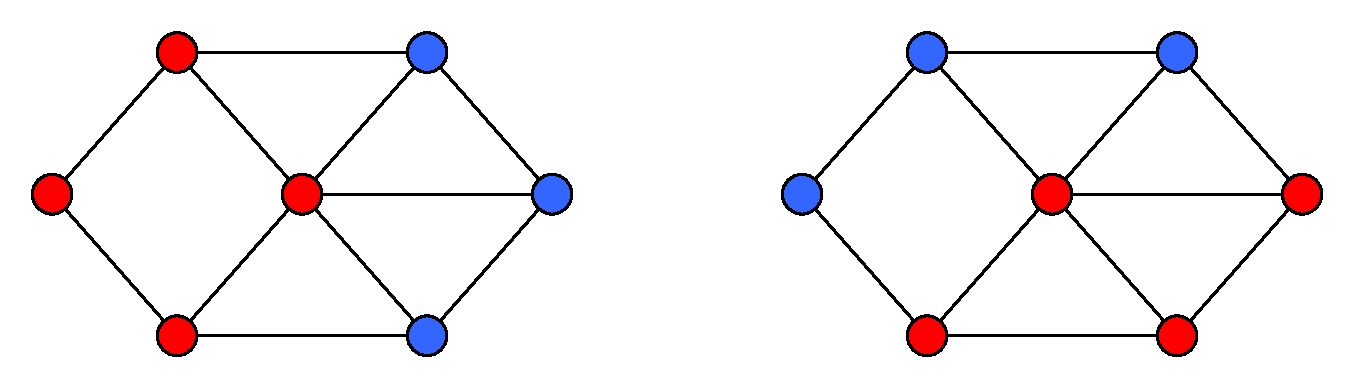
\includegraphics[scale=0.35]{chapter2/fig/badpartition.pdf}
	\caption[Example of bad partition of two equal graphs]{Example of bad partition of two equal graphs. Since clusters are very different, their matching in all possible combinations will always have low quality.} \label{fig:badpartition}
\end{figure}

To cope with such problems, we formulated our method as an iterative process. After each iteration the subgraphs of the initial graphs have a chance to exchange nodes with their neighbors based on the obtained solution $m$ and improve the matching quality of the next iteration. The proposed updating process consists of two major steps. In the first step we estimate an affine transformation between matched subgraphs based on the provided local correspondences. The next step is the actual update step, where the updating process uses the estimated transformations.
We explain our approach on a pair of matched subgraphs $G[V^I_k]=(V^I_k, E^I_k, D^I_k)$ and $G[V^J_p]=(V^J_p, E^J_p, D^J_p)$  with the obtained local correspondence set $m^{kp}=\{(v_i,v_j)|v_i\in V^I_k, v_j\in V^J_p\}$. 

In the first step we want to estimate two affine transformations $T_{kp}:V^I_k\rightarrow V^J_p$ and $T_{pk}:V^J_p\rightarrow V^I_k$ from the node set of one subgraph into another and vice versa. For that we use the state-of-the-art Coherent Point Drift~(CPD) algorithm by Myronenko and Song~\cite{Myronenko2009_CPD}. This is an probabilistic algorithm for the points set registration problem, which finds correspondences between two set of points and a transformation that describes the mapping between the sets. We choose it, because it shows a remarkable robustness against outliers and often outperforms the other popular algorithm TPS-RPM by Chui and Rangarajan~\cite{Chui2003}, which we mentioned in chapter~\ref{chapter:GM}. After obtaining the affine transformations $T_{kp}$ and $T_{pk}$ we measure a transformation error of each matched node $v_i\in V^I_k (v_j\in V^J_k)$ as a distance between its projection into the other subgraph $T_{kp}(v_i) (T_{pk}(v_j))$ and its matched pair $m(v_i) = v_j\in V^J_p\ (m(v_j) = v_i\in V^I_k)$:
\begin{align}\begin{split} \label{eq:err_v}
err(v_i) &= \|T_{kp}(v_i) - m(v_i)\|_{2}\\
err(v_j) &= \|T_{pk}(v_j) - m(v_j)\|_{2}
\end{split}\end{align}
Based on the errors of single nodes we assign an error to the estimated transformations as a measure of their quality:
\begin{equation}\begin{split} \label{eq:err_T}
err(T_{kp}) & = \median_{v_i\in V^I_k}err(v_i) \\
err(T_{pk}) & = \median_{v_j\in V^J_p}err(v_j)
\end{split}\end{equation}
From both transformations we select the one with the smallest error and replace the second with the inverse transformation of the selected one. For simplicity we preserve the notation $T_{kp}$ and $T_{pk}$ for the transformations related to the subgraph match $(a_k, a_p)$. In this way we associate with each pair of matched subgraphs, that have at least $3$ provided node correspondences\footnote{We need at least $3$ pairs of correspondences between two sets of points to be able to estimate an affine transformation between them.}, two affine transformations between their nodes.

In the next step, we apply the estimated transformations to each subgraph of both graphs to project them into the node space of the opposite graph (see Fig.~\ref{fig:update}). For the subgraph $G[V^J_p]$ that means, that the transformation $T_{pk}$ associated with the anchor pair $(a_k,a_p)$ is now casted as a mapping $T_{pk}:V^J_p\rightarrow V^I$. For the projected points $T_{pk}(v_j),v_j\in V^J_p,$ we find their nearest neighbors $\bar{v}_i=NN(T_{pk}(v_j))$ in $V^I$. In Fig.~\ref{fig:update} the projected points $T_{pk}(v_j),v_j\in V^J_p,$ are marked with bright red color. We define a new matrix $\bar{U}^{Ia}\in\mathbb{R}^{|V^I|\times m_1}$ and assign to its elements $\bar{U}^{Ia}_{\bar{v}_i,a_k}=\|T_{pk}(v_j)-\bar{v}_i\|_2$ the distance between the projections $T_{pk}(v_j)$ of $v_j\in V^J_p$ and their nearest neighbor $NN(T_{pk}(v_j))$ in $V^I$.

\begin{figure}[h]
	\centering
	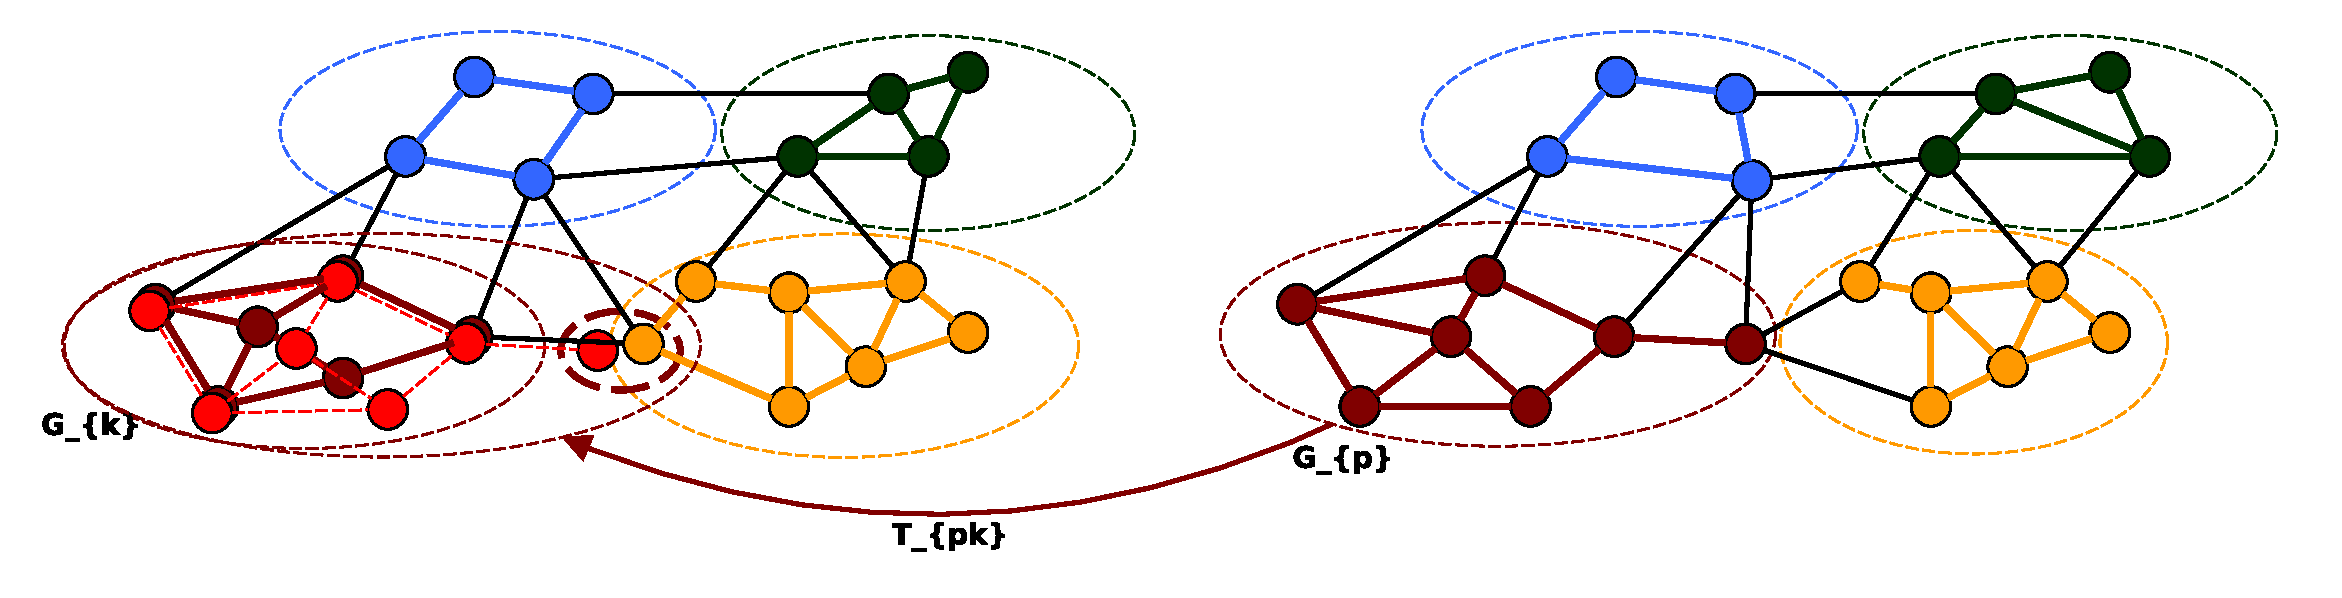
\includegraphics[scale=0.35]{chapter2/fig/update.pdf}
	\caption{Example of the graph partition update rule} \label{fig:update}
\end{figure}

After performing the same procedure for all transformations $T_{pk}$ we set all not-assigned elements of $\bar{U}^{Ia}$ to infinite. If there are some lines in $\bar{U}^{Ia}$ where all elements equal are infinite, meaning that the corresponding nodes in $V^I$ are not selected as nearest neighbors of the projections of the nodes in $V^J$,
then we replace those lines with the corresponding lines in the current matrix $U^{Ia}$ (see definition~\eqref{eq:matrixU}).

Our update rule for the partition of the graph $G^I$ defined by the matrix $U^{Ia}$ is:
\begin{equation}
U^{Ia}_{ik}=1 \iff a_k=\argmin_{l=1,\dots,m_1}^{}{\bar{U}^{Ia}_{v_i,a_l}}
\end{equation}
With the other words, the node $v_i\in V^I$ is assigned to the anchor $a_k$ if $\bar{U}_{v_i,a_k}$ is the smallest distance between $v_i$ and projections of the nodes in the subgraphs $G[V^J_p]$ matched to the subgraph $G[V^I_k]$. Note, that unassigned nodes in $V^I$ stay in the same cluster where they were before. It also can happen, that one note on different iterations will be assigned to different clusters. This can be often the case on the border between two good estimated clusters. To prevent unnecessary jumps, we introduce a local memory of each node, where it saves information about clusters it belonged to and associated value of the matrix $\bar{U}^{Ia}$. We assign a node to a new cluster only when a new assignment is better than the previous ones.

The partition of the second graph is updated in the same way, as it is described above for the graph $G^I$. The approach is summarized in Algorithm~\ref{alg:update_subgraphs4.3.2}.

\begin{algorithm}[h]
	\KwIn{  $m^a = \{(a_k, a_p)|a_k\in V^{Ia}, a_p\in V^{Ja}\}$\\
		\hspace{45pt}$m = \{(v_i, v_j)|v_i\in V^{I}, v_j\in V^{J}\}$}
	\KwOut{updated $U^{Ia}$, $U^{Ja}$}
	\tcc{Step $1$: assign affine transformations to each pair $(a_k, a_p)$ } 
	\ForEach{matched subgraph pair $(a_k, a_p)$}
	{
		calculate $T_{kp}:V^I_k\rightarrow V^J_p$ and $T_{pk}:V^J_p\rightarrow V^I_k$ using CPD algorithm
	}
	\tcc{Step $2$: calculate new matrices $\bar{U}^{Ia}\in\mathbb{R}^{|V^I|\times m_1}$, $\bar{U}^{Ja}\in\mathbb{R}^{|V^J|\times m_2}$ }
	\ForEach{matched subgraph pair $(a_k, a_p)$}
	{
		$\forall v_j\in V^J_p:\quad$ $\bar{U}^{Ia}_{\bar{v}_i,a_k}=\|T_{pk}(v_j)-\bar{v}_i\|_2$, where $\bar{v}_i=NN(T_{pk}(v_j))\in V^I$\\
		$\forall v_i\in V^I_k:\quad$ $\bar{U}^{Ja}_{\bar{v}_j,a_p}=\|T_{kp}(v_i)-\bar{v}_j\|_2$, where $\bar{v}_j=NN(T_{kp}(v_i))\in V^J$
	}
	\tcc{Step $3$: update partitions}
	$U^{Ia}_{ik}=1 \iff a_k=\argmin_{l=1,\dots,m_1}^{}{\bar{U}^{Ia}_{v_i,a_l}}$\\
	$U^{Ja}_{jp}=1 \iff a_p=\argmin_{q=1,\dots,m_2}^{}{\bar{U}^{Ja}_{v_j,a_q}}$\\
	\Return $U^{Ia}$, $U^{Ja}$
	
	\caption{UpdateSubgraphs}    \label{alg:update_subgraphs4.3.2}
\end{algorithm}

The usage of the proposed graph partition strategy is illustrated in Fig.~\ref{fig:update}. After performing the update procedure, the most left yellow node is likely to be included in the red partition, where in fact it should belong to.
\FloatBarrier
% ---------------------------------------        Complexity
\subsection{Complexity}
We would like to investigate the \ToDo{asymptotic computational} complexity of our two level graph matching approach. For simplicity, we assume, that the complexity of a selected graph matching algorithm is $\mathcal{O}(f_{GM}(n_1,n_2))$, where $n_1$ and $n_2$ are the size of the graphs we want to match.

The preprocessing step of our approach consists of two stages: initial graph partitioning and creation of the codebook of the node attributes. Note that the presence of the second stage depends on the selected strategy of the anchor graph matching. The complexity of the graph partitioning is in the worst case equal to $\mathcal{O}(n_2^2)$\footnote{We assumed $n_1\le n_2$}. Indeed, for one graph with $n$ nodes and $m$ anchors it is equal to $\mathcal{O}(nm)$ (using grid approach) or $\mathcal{O}((n-m)\Delta(G))$\footnote{We denote with $\Delta(G)$ the maximal degree of nodes in $V$, where degree of a node is equal to the number of its incident edges~\cite{Diestel2000}.} (HEM or LEM algorithm). The complexity of the codebook creation is determined by the complexity of the clustering algorithm, which in case of Lloyd's k-means algorithm~\cite{kmeans_LLoyd} comes to $\mathcal{O}((n_1+n_2)rC)$ per iteration, where $r$ is the dimension of the node attribute vectors and $C$ the number of clusters. After joining those two results we obtain that the complexity of the preprocessing step is
\begin{equation}\label{eq:complexity1}
\mathcal{O}(n_2^2+(n_1+n_2)rCi),
\end{equation}where $i$ is the maximum number of iterations of the k-means clustering.

The main loop of our two level graph matching approach consists of three steps. The first one is the anchor graph matching, whose complexity is $\mathcal{O}(f_{GM}(m_1,m_2))$ plus the complexity for initialization of the similarity matrix. In case, when we assign attributes to the anchors to calculate node similarity between two graphs, the complexity of the initialization can be approximated by $\mathcal{O}(m_1^2m_2^2)$. The complexity of the subgraph matching step afterwards results in $\sum_{(a_k,a_p)\in m^a}\mathcal{O}(f_{GM}(|V^I_k|,|V^J_p|))$. The complexity of the two first steps in this case is equal to
\begin{equation}\label{eq:complexity2}
\mathcal{O}(m_1^2m_2^2)+\mathcal{O}(f_{GM}(m_1,m_2))+\sum_{(a_k,a_p)\in m^a}\mathcal{O}(f_{GM}(|V^I_k|,|V^J_p|)).
\end{equation}

In the case, when we use graph matching to determine the similarity between anchors, the complexity of both anchor and subgraph matching is equal to 
\begin{equation}
\sum_{(a_k,a_p)\in M^a}\mathcal{O}(f_{GM}(|V^I_k|,|V^J_p|)),\quad M^a=\{(a_k,a_p)|a_k\in V^{Ia},a_p\in V^{Ja}\},
\end{equation}because subgraph matching is already included in the anchor matching step.

At the end we only need to determine the complexity of our update rule. The CPD algorithm has linear complexity, which means we can estimate transformations between all matched subgraphs with demand $\sum_{(a_k,a_p)\in M^a}\mathcal{O}(\max(|V^I_k|,|V^J_p|))$. The actual update step afterwards has the complexity $\mathcal{O}(n_1m_1+n_2m_2)$.

If we assume, that we can completely parallelize the computation of the sum in Eq.~\eqref{eq:complexity2}, that the total complexity of one iteration of our two level graph matching approach is equal to
\begin{equation}\label{eq:complexity3}
\begin{split}
\mathcal{O}(m_1^2m_2^2)&+\mathcal{O}(f_{GM}(m_1,m_2))+\mathcal{O}(f_{GM}(\max_{k}|V^I_k|,\max_{p}|V^J_p|))\\
                       &+\mathcal{O}(f_{GM}(\max_{k}|V^I_k|,\max_{p}|V^J_p|))+\mathcal{O}(n_1m_1+n_2m_2)
\end{split}
\end{equation}
or
\begin{equation}\label{eq:complexity4}
\begin{split}
\mathcal{O}(m_1^2m_2^2)&+\mathcal{O}(f_{GM}(m_1,m_2))+\mathbf{m_2}\mathcal{O}(f_{GM}(\max_{k}|V^I_k|,\max_{p}|V^J_p|))\\
&+\mathcal{O}(f_{GM}(\max_{k}|V^I_k|,\max_{p}|V^J_p|))+\mathcal{O}(n_1m_1+n_2m_2)
\end{split}
\end{equation}
depending on the selected strategy for computing the similarity between anchor graphs. Let us notice that the constant $m_2$ in Eq.~\eqref{eq:complexity4} increases the complexity of the whole algorithm, when we use subgraph matching to calculate the similarity between anchors.

However, because of the complexity of the graph matching is the most expensive (in case of RRWM $\mathcal{O}(f_{GM}(n_1,n_2))=\mathcal{O}(n_1^2n_2^2)$), it will fully beat the complexity of other steps and we can approximate both Eqs.~\eqref{eq:complexity3} and~\eqref{eq:complexity4} with
\begin{equation}\label{eq:complexity3.1}
\mathcal{O}(f_{GM}(m_1,m_2))+\mathcal{O}(f_{GM}(\max_{k}|V^I_k|,\max_{p}|V^J_p|))
\end{equation} 
and 
\begin{equation}\label{eq:complexity4.1}
\mathcal{O}(f_{GM}(m_1,m_2))+\mathbf{m_2}\mathcal{O}(f_{GM}(\max_{k}|V^I_k|,\max_{p}|V^J_p|))
\end{equation}
respectively.

It is obvious, that the resulting complexity of our graph matching framework depends highly on the number of iterations and on the size of the anchor graphs and subgraphs.


% -------------------------  Discussion ----------------------------------------------------------------------
\section{Discussion}
We have proposed a novel framework for solving a graph matching problem formulated as an quadratic assignment problem. Our framework is based on a known matching algorithm, but helps to cope with some limitations of its application, such as big space demand and high computation time.
%Our framework does not represent a new matching algorithm, but helps an existing one to cope with some limitations of it application, such as big space demand and high computational time.
Its core idea of the introduces framework is to decompose an initial graph matching problem into a set of subproblems. For that we partition graphs into subgraphs, perform matching to determine pairs of subgraphs and afterwards perform matching again for each pair of subgraphs. An obtained solution at the end is used to update the graph partition. The whole procedure is repeated iteratively until it converges. The complexity of the proposed method depends highly on the complexity of the used graph matching algorithm, which in its turn depends on the size of the anchor graph and the graph subgraphs. In the next chapter we evaluate the proposed framework on synthetic and real data examples.
%\ToDo{In the next chapter we apply the proposed framework to synthetic and real data examples.}